\chapter{坐标系与矢量分析\label{chapter:reference}}

%%%%%%%%%%%%%%%%%%%%%%%%%%%%%%%%%%%%%%%%%%%%%%%%%%%%%%%%%%%%%%%%%%%%%
\section{Cartesian坐标系与矢量\label{section:reference-cartesian}}
%%%%%%%%%%%%%%%%%%%%%%%%%%%%%%%%%%%%%%%%%%%%%%%%%%%%%%%%%%%%%%%%%%%%%

\subsection{坐标系}
Cartesian坐标系是直角坐标系和斜坐标系的统称。我们一般讨论的是直角坐标系,有二维的$xy$
坐标系和三维的$xyz$坐标系,这些坐标系下,每个轴都互相垂直。
\begin{figure}[h]
    \centering
    \setlength{\abovecaptionskip}{0.2cm}
    \inkfig{0.6}{./figure/math/CartesianCoord.pdf_tex}
    \caption{二维直角坐标系和三维直角坐标系}
    \label{fig:CartesianCoord}
\end{figure}

\subsection{矢量分析}
\begin{definition}[标量和矢量]
    标量指有大小无方向的量;矢量指有大小有方向的量。 
\end{definition}
常见的标量有温度、湿度、质量、电荷等;矢量有位移、速度、电场等。定义沿$x$、$y$和$z$轴
方向的单位矢量为$\vbe_x$、$\vbe_y$和$\vbe_z$。

\paragraph*{矢量操作}
\begin{enumerate}
    \item \textit{矢量加法}:矢量$\vbB$的尾叠在矢量$\vbA$的头上。一般表现为三角形
          规则或平行四边形规则。满足交换律和集合律
          \begin{align}
              \vbA + \vbB &= \vbB + \vbA
                                          \label{eq:vec-vec-add-exchang} \\
              \vbA + (\vbB + \vbC) &= (\vbA + \vbB) + \vbC
                                          \label{eq:vec-vec-add-combine}
          \end{align}
    \item \textit{标量与矢量乘法}:正值标量与矢量相乘只改变矢量大小不改变方向,负值标
          量与与矢量相乘改变矢量的大小和方向,$0$与矢量相乘永远标量为0。满足分配律
          \begin{equation}
              \begin{aligned}
                  a(\vbA + \vbB) &= a\vbA + a\vbB \\
                  (a + b) \vbA     &= a\vbA + b\vbA
              \end{aligned}
            \label{eq:vec-distri}
          \end{equation}
    \item \textit{矢量与矢量点积}:两矢量点积定义为
           \begin{equation}
               \vbA \cdot \vbB = |\vbA|\ |\vbB|\cos{\theta}
            \label{eq:vec-dotproduct}
           \end{equation}
           $\theta$为$\vbA$与$\vbB$之间的夹角。满足交换律和分配律
           \begin{align}
               \vbA \cdot \vbB &= \vbB \cdot \vbA
                                           \label{eq:vec-vec-dot-exchange}   \\
               \vbA \cdot (\vbB + \vbC) &= \vbA \cdot \vbB + \vbA \cdot \vbB
                                           \label{eq:vec-vec-dot-distri}
           \end{align}
    \item \textit{矢量与矢量叉积}:两矢量叉积定义为
          \begin{equation}
              \vbA \times \vbB = |\vbA|\ |\vbB|\sin{\theta} \hat{\vbn}
            \label{eq:vec-vec-cross}
          \end{equation}
          $\theta$为$\vbA$与$\vbB$之间的夹角,$\hat{\vbn}$为同时垂直与$\vbA$和$\vbB$的单
          位矢量。满足分配律
          \begin{equation}
              \vbA \times(\vbB + \vbC) = \vbA \times \vbB + \vbA \times \vbC
                                            \label{eq:vec-vec-cross-distri}
          \end{equation}
          不满足交换律,但有
          \begin{equation}
              \vbA \times \vbB = - \vbB \times \vbA
            \label{eq:vec-vec-cross-exchange}
          \end{equation}
          $\vbA$与$\vbB$的叉积可理解为边长为$A$和$B$的平行四边形的面积,在乘上此
          四边形法向的单位向量。
      \item \textit{混合积1}:
            \begin{equation}
                \begin{aligned}
                    (\vbA \times \vbB) \cdot \vbC 
                                        =& (\vbB \times \vbC) \cdot \vbA \\
                                        =& (\vbC \times \vbA) \cdot \vbB \\
                                        =&-(\vbB \times \vbA) \cdot \vec{C} \\
                                        =&-(\vbC \times \vbB) \cdot \vbA \\
                                        =&-(\vbA \times \vbC) \cdot \vbB \\
                \end{aligned}
                \label{eq:vec-vec-vec-mix1}
            \end{equation}
            \CJKunderdot{注意}:上式第一个等号右边的乘积顺序是
            $\vbA \rightarrow \vbB \rightarrow \vbC$,前两个等号右边式子从$\vbA$开始也遵
            循同样的规律,因此其前面符号为正;最后三个等号从$\vec{A}$开始的顺序为
            $\vbA \rightarrow \vbC \rightarrow \vbB$,顺序不再与第一个式子相同,
            出现负号。
      \item \textit{混合积2}:
          \begin{equation}
          \vbA \times (\vbB \times \vbC) = \vbB(\vbA \cdot \vbC) - \vbC(\vbA \cdot \vbB)
                                                        \label{eq:vec-vec-vec-mix2}
          \end{equation}
\end{enumerate}

三维直角坐标系沿坐标轴正方向定义三个正交的单位矢量$\vbe_x$、$\vbe_y$和$\vbe_z$,
他们之间的关系为
\begin{equation}
    \begin{aligned}
        \vbe_{i} \cdot  \vbe_{j} =& \delta_{ij} \\
        \vbe_{i} \times \vbe_{j} =& \epsilon_{ijk} \vbe_{k}
    \end{aligned}
    \label{eq:vec-cartesian}
\end{equation}
$\epsilon_{ijk}$为Levi-Civita符号,是一三阶反对称张量,满足
\begin{equation}
    \begin{aligned}
        \epsilon_{ijk} =& - \epsilon_{jik} = -\epsilon_{ikj} \\
        \epsilon_{123} =& 1
    \end{aligned}
    \label{eq:Levi-Civita}
\end{equation}
角坐标系中任一矢量都可由这三个单位矢量经线性组合构成,进而定义矢量与矢量、矢量与标
量间的运算规则。

%%%%%%%%%%%%%%%%%%%%%%%%%%%%%%%%%%%%%%%%%%%%%%%%%%%%%%%%%%%%%%%%%%%%%
\subsection{矢量运算}
\paragraph*{导数}
对于一个单变量函数$f(x)$,它的导数$\mathrm{d} f(x)/ \mathrm{d} x$表明它变化的快慢
\begin{equation}
    \mathrm{d} f = \frac{\mathrm{d} f}{\mathrm{d} x} dx
                                \label{eq:vec-derivative}
\end{equation}
上式可以表示为当$x$变化为$\mathrm{d}x$时,$f$变化为$\mathrm{d}f$,而导数则是这两个变
化值间的一个因子。几何上则将导数解释为$f$对$x$的斜率。

\paragraph*{$\nabla$算符}
定义$\nabla$算符为
\begin{equation}
    \nabla =    \vbe_x \frac{\partial}{\partial x} 
               +\vbe_y \frac{\partial}{\partial y}
               +\vbe_z \frac{\partial}{\partial z}
    \label{eq:nabla-operator}
\end{equation}
$\nabla$算符本身具有矢量的特性,但若不作用在函数上的话这个符号就没有任何意义。有三种
作用方式:
\begin{enumerate}
    \item 作用于一个标量函数$T$上:$\nabla T$(梯度)
    \item 通过点积作用到矢量函数$\vec{v}$上:$\nabla \cdot \vec{v}$(散度)
    \item 通过叉积作用到矢量函数$\vec{v}$上:$\nabla \times \vec{v}$(旋度)
\end{enumerate}

\paragraph*{梯度}
梯度是针对标量函数$T$,它的梯度是单变量导数的推广,写为
\begin{equation}
    \nabla T =   \frac{\partial T}{\partial x}\vbe_x 
               + \frac{\partial T}{\partial y}\vbe_y
               + \frac{\partial T}{\partial z}\vbe_z
    \label{eq:vec-gradient}
\end{equation}
\uline{梯度具有大小和方向}。梯度$\nabla T$所指方向是函数$T$具有最大增加的方向,
$|\nabla T|$代表这个最大增加方向的斜率。同样的,梯度为$0$标志着极大、极小或平直。

\CJKunderdot{有关梯度的基本定理}:对一个三变量的标量函数$T(x, y, z)$,从$a$点出发,
选定任意一条路径$P$,每次移动一个微小位移,直至最后到达点$b$,那么$T$沿着这个路径的
总改变量为
\begin{equation}
    \int_{a}^{b} (\nabla T) \cdot \mathrm{d} \vec{l}_{P} = T(b) - T(a)
    \label{eq:vec-gradiant-basictheorem}
\end{equation}
从式\eqref{eq:vec-gradiant-basictheorem}可看出,该路径积分只与路径始末端有关,而与路
径无关。从中可得到两个推论:
\begin{itemize}
    \item \textit{推论1}:梯度的路径积分只与路径边界值相关而与所选路径无关;
    \item \textit{推论2}:当所选路径闭合时,梯度对该路径的积分为零。
\end{itemize}

\paragraph*{散度}
散度是针对矢量函数的,一个标量函数的散度是无意义的。一个矢量函数$\vec{v}(x, y, z)$的
散度是一个标量
\begin{equation}
    \nabla \cdot \vbv = (   \vbe_x \frac{\partial T}{\partial x} 
                             + \vbe_y \frac{\partial T}{\partial y}
                             + \vbe_z \frac{\partial T}{\partial z})
                           \cdot
                           (\vbv_x + \vbv_y + \vbv_z)
    \label{eq:vec-devergence}
\end{equation}

\uline{几何解释}:散度是指矢量场在某一点出散出的量度,描述的是发散的程度,而发散是具
有方向的一个动作,因而散度是针对矢量而言的。具体如下图所示
\begin{figure}[ht]
    \centering
    \setlength{\abovecaptionskip}{0.2cm}
    \subfloat[]{
        \begin{tikzpicture}
    \draw[-Stealth, line width=1pt]             (0, 0) -- (0.8, 0);
    \draw[-Stealth, line width=1pt, rotate=30]  (0, 0) -- (0.8, 0);
    \draw[-Stealth, line width=1pt, rotate=60]  (0, 0) -- (0.8, 0);
    \draw[-Stealth, line width=1pt, rotate=90]  (0, 0) -- (0.8, 0);
    \draw[-Stealth, line width=1pt, rotate=120] (0, 0) -- (0.8, 0);
    \draw[-Stealth, line width=1pt, rotate=150] (0, 0) -- (0.8, 0);
    \draw[-Stealth, line width=1pt, rotate=180] (0, 0) -- (0.8, 0);
    \draw[-Stealth, line width=1pt, rotate=210] (0, 0) -- (0.8, 0);
    \draw[-Stealth, line width=1pt, rotate=240] (0, 0) -- (0.8, 0);
    \draw[-Stealth, line width=1pt, rotate=270] (0, 0) -- (0.8, 0);
    \draw[-Stealth, line width=1pt, rotate=300] (0, 0) -- (0.8, 0);
    \draw[-Stealth, line width=1pt, rotate=330] (0, 0) -- (0.8, 0);

    \draw[-Stealth, line width=1pt]             (1, 0) -- (2.5, 0);
    \draw[-Stealth, line width=1pt, rotate=30]  (1, 0) -- (2.5, 0);
    \draw[-Stealth, line width=1pt, rotate=60]  (1, 0) -- (2.5, 0);
    \draw[-Stealth, line width=1pt, rotate=90]  (1, 0) -- (2.5, 0);
    \draw[-Stealth, line width=1pt, rotate=120] (1, 0) -- (2.5, 0);
    \draw[-Stealth, line width=1pt, rotate=150] (1, 0) -- (2.5, 0);
    \draw[-Stealth, line width=1pt, rotate=180] (1, 0) -- (2.5, 0);
    \draw[-Stealth, line width=1pt, rotate=210] (1, 0) -- (2.5, 0);
    \draw[-Stealth, line width=1pt, rotate=240] (1, 0) -- (2.5, 0);
    \draw[-Stealth, line width=1pt, rotate=270] (1, 0) -- (2.5, 0);
    \draw[-Stealth, line width=1pt, rotate=300] (1, 0) -- (2.5, 0);
    \draw[-Stealth, line width=1pt, rotate=330] (1, 0) -- (2.5, 0);
\end{tikzpicture}

        \label{fig:vec-diverg-a}
    }
    \hfill
    \subfloat[]{
        \begin{tikzpicture}
    \draw[-Stealth, line width=1pt]               (0.0, 0.0) -- (0.0, 2.0);
    \draw[-Stealth, line width=1pt]               (0.0, 2.2) -- (0.0, 4.2);
    \draw[-Stealth, line width=1pt]               (0.6, 0.8) -- (0.6, 2.8);
    \draw[-Stealth, line width=1pt]               (0.6, 3.0) -- (0.6, 5.0);

    \draw[-Stealth, line width=1pt, xshift=1.2cm] (0.0, 0.0) -- (0.0, 2.0);
    \draw[-Stealth, line width=1pt, xshift=1.2cm] (0.0, 2.2) -- (0.0, 4.2);
    \draw[-Stealth, line width=1pt, xshift=1.2cm] (0.6, 0.8) -- (0.6, 2.8);
    \draw[-Stealth, line width=1pt, xshift=1.2cm] (0.6, 3.0) -- (0.6, 5.0);

    \draw[-Stealth, line width=1pt, xshift=2.4cm] (0.0, 0.0) -- (0.0, 2.0);
    \draw[-Stealth, line width=1pt, xshift=2.4cm] (0.0, 2.2) -- (0.0, 4.2);
    \draw[-Stealth, line width=1pt, xshift=2.4cm] (0.6, 0.8) -- (0.6, 2.8);
    \draw[-Stealth, line width=1pt, xshift=2.4cm] (0.6, 3.0) -- (0.6, 5.0);

    \draw[-Stealth, line width=1pt, xshift=3.6cm] (0.0, 0.0) -- (0.0, 2.0);
    \draw[-Stealth, line width=1pt, xshift=3.6cm] (0.0, 2.2) -- (0.0, 4.2);
    \draw[-Stealth, line width=1pt, xshift=3.6cm] (0.6, 0.8) -- (0.6, 2.8);
    \draw[-Stealth, line width=1pt, xshift=3.6cm] (0.6, 3.0) -- (0.6, 5.0);
\end{tikzpicture}

        \label{fig:vec-diverg-b}
    }
    \hfill
    \subfloat[]{
        \begin{tikzpicture}
    \draw[-Stealth, line width=1pt]               (0.0, 0.0) -- (0.0, 1.0);
    \draw[-Stealth, line width=1pt]               (0.0, 1.2) -- (0.0, 2.5);
    \draw[-Stealth, line width=1pt]               (0.0, 2.7) -- (0.0, 5.0);

    \draw[-Stealth, line width=1pt, xshift=0.6cm] (0.0, 0.0) -- (0.0, 1.0);
    \draw[-Stealth, line width=1pt, xshift=0.6cm] (0.0, 1.2) -- (0.0, 2.5);
    \draw[-Stealth, line width=1pt, xshift=0.6cm] (0.0, 2.7) -- (0.0, 5.0);

    \draw[-Stealth, line width=1pt, xshift=1.2cm] (0.0, 0.0) -- (0.0, 1.0);
    \draw[-Stealth, line width=1pt, xshift=1.2cm] (0.0, 1.2) -- (0.0, 2.5);
    \draw[-Stealth, line width=1pt, xshift=1.2cm] (0.0, 2.7) -- (0.0, 5.0);

    \draw[-Stealth, line width=1pt, xshift=1.8cm] (0.0, 0.0) -- (0.0, 1.0);
    \draw[-Stealth, line width=1pt, xshift=1.8cm] (0.0, 1.2) -- (0.0, 2.5);
    \draw[-Stealth, line width=1pt, xshift=1.8cm] (0.0, 2.7) -- (0.0, 5.0);

    \draw[-Stealth, line width=1pt, xshift=2.4cm] (0.0, 0.0) -- (0.0, 1.0);
    \draw[-Stealth, line width=1pt, xshift=2.4cm] (0.0, 1.2) -- (0.0, 2.5);
    \draw[-Stealth, line width=1pt, xshift=2.4cm] (0.0, 2.7) -- (0.0, 5.0);

    \draw[-Stealth, line width=1pt, xshift=3.0cm] (0.0, 0.0) -- (0.0, 1.0);
    \draw[-Stealth, line width=1pt, xshift=3.0cm] (0.0, 1.2) -- (0.0, 2.5);
    \draw[-Stealth, line width=1pt, xshift=3.0cm] (0.0, 2.7) -- (0.0, 5.0);

    \draw[-Stealth, line width=1pt, xshift=3.6cm] (0.0, 0.0) -- (0.0, 1.0);
    \draw[-Stealth, line width=1pt, xshift=3.6cm] (0.0, 1.2) -- (0.0, 2.5);
    \draw[-Stealth, line width=1pt, xshift=3.6cm] (0.0, 2.7) -- (0.0, 5.0);
\end{tikzpicture}

        \label{fig:vec-diverg-c}
    }
    \caption{}
    \label{fig:vec-diverg}
\end{figure}
\newline
图\ref{fig:vec-diverg-a}中,在给定点处只有穿出的矢量,因此具有较大的正值散度(箭头外
指为正,内指为负);图\ref{fig:vec-diverg-b}中,取定某一点,穿入该点和穿出该点的矢量
的度量是一样的,因此其的散度为0;图\ref{fig:vec-diverg-c}中,取定某一点,穿入该点的
矢量比穿出该点的矢量的度量要小,因此具有正的散度。

\CJKunderdot{有关散度的基本定理}:散度定理又称为高斯定理、格林定理,表示为
\begin{equation}
    \int_{V} (\nabla \cdot \vbv)\ \mathrm{d} \tau
                         = \oint_{S} \vbv \cdot \mathrm{d} \vba
    \label{eq:div-basetheo}
\end{equation}
它指出,一个矢量函数散度在区域的体积分可以转化该矢量函数在该区域边界上的面积分值。我
们可将$\vbv$当成一个不可压缩的流,$\vbv$的通量是单位时间内流出表面的总流量
(式\eqref{eq:div-basetheo}左边)。某点处$\vbv$的散度表示该点产生或吸收流的量度(散度为正表
示放出流,散度为负表示吸收流),对于空间中某一区域,其在单位时间内产生(或吸收)的流等于流经
其表面的通量。


\paragraph*{旋度}
旋度只针对矢量,标量的旋度没有任何意义,矢量的旋度仍为一个矢量。对矢量$\vec{v}(x, y, z)$
的旋度定义为
\begin{equation}
    \nabla \times \vbv = 
    \left|\begin{matrix}
        \vbe_x               &   \vbe_y               &   \vbe_z   \\
        \partial / \partial x   &   \partial / \partial y   &   \partial / \partial y  \\
        v_x                     &   v_y                     &   v_z 
    \end{matrix}\right|
    \label{eq:vec-curl}
\end{equation}

\uline{几何解释}:旋度表示在所选点处漩涡状态的量度,按右手规则确定旋度的方向。如图中
所示的旋度就不为零。旋度很常见,比如大海中的漩涡。
\begin{figure}[ht]
    \centering
    \setlength{\abovecaptionskip}{0.2cm}
    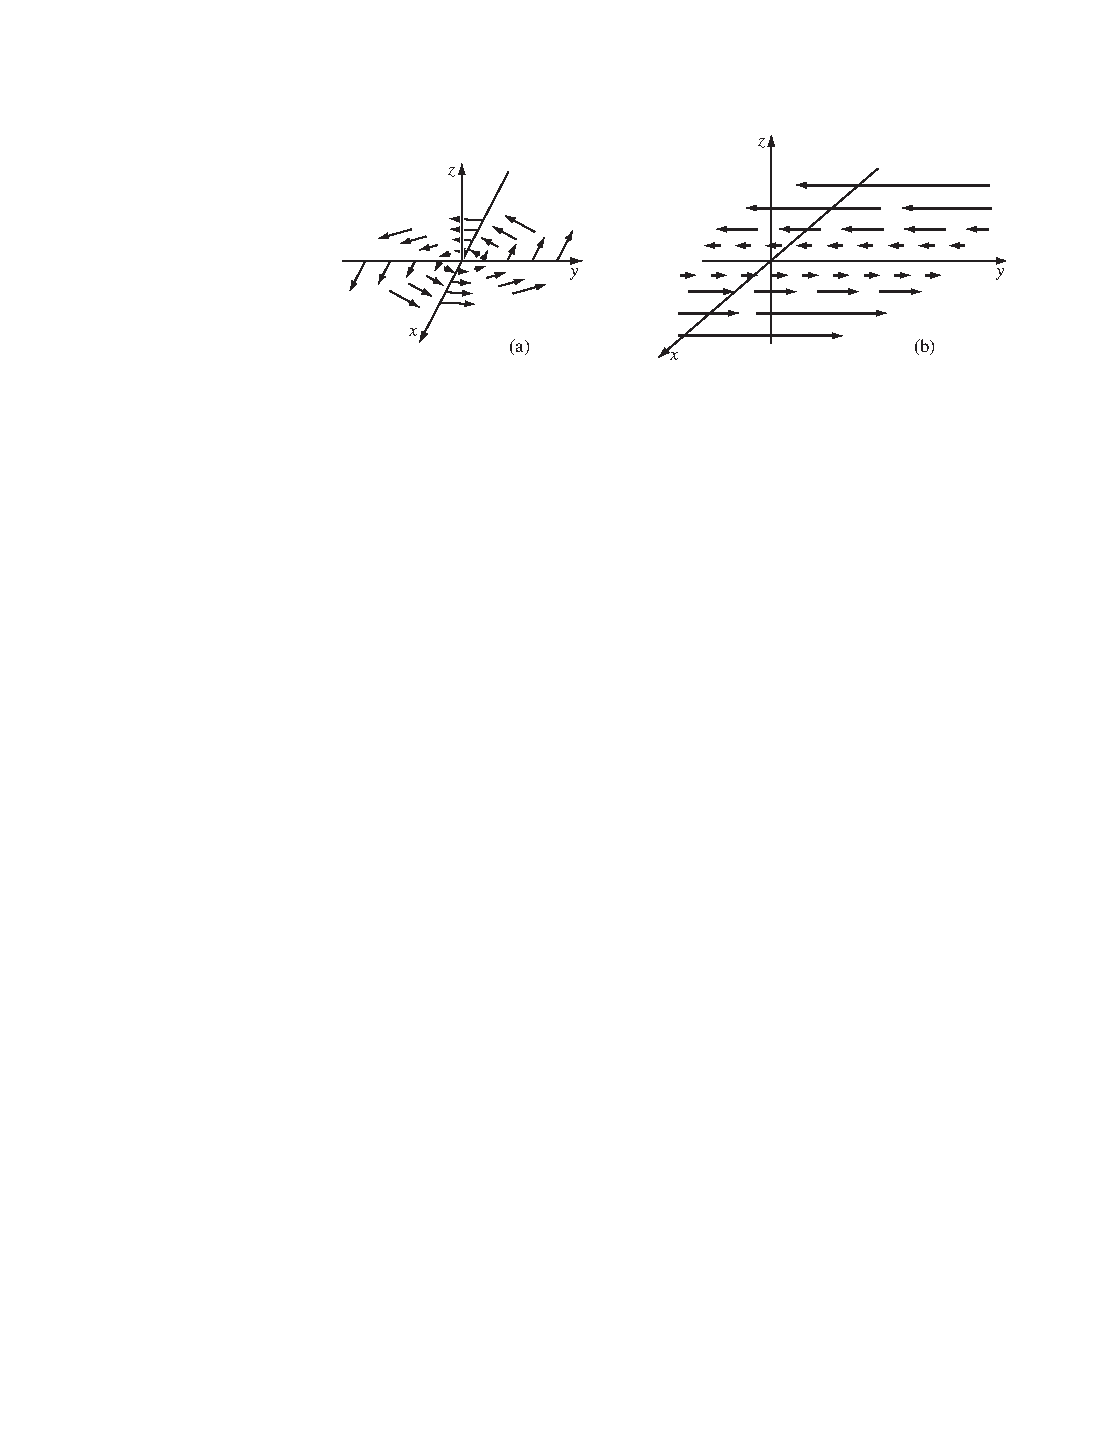
\includegraphics[scale=1.3]{./figure/math/vec-curl.pdf}
    \caption{}
    \label{fig:vec-curl}
\end{figure}

\subsection{积规则}
针对$\nabla$算符,标量由两种方式构建:
\begin{center}
    $fg$ \\
    $\vbA\vbB$
\end{center}
矢量由两种方式构建:
\begin{center}
    $f\vbA$ \\
    $\vbA \times \vbB$
\end{center}

%%%%%%%%%%%%%%%%%%%%%%%%%%%%%%%%%%%%%%%%%%%%%%%%%%%%%%%%%%%%%%%%%%%%
\section{极坐标系\label{section:reference-polar}}
%%%%%%%%%%%%%%%%%%%%%%%%%%%%%%%%%%%%%%%%%%%%%%%%%%%%%%%%%%%%%%%%%%%%%
点$P$的位置在二维直角坐标系中用相互垂直的两个轴线的具体值$P(x, y)$表示,在极坐标中则
用两个不相干的参数$P(r, \theta)$表示,如下图:
如图\ref{fig:PolarCoord}。
\begin{figure}[ht]
    \centering
    \setlength{\abovecaptionskip}{0.2cm}
    \begin{tikzpicture}
    \draw[-Stealth, line width=1pt](0, 0) -- (4, 0);
    \node at (3.8, -0.2) {$x$};
    \draw[-Stealth,color=gray](0, 0) -- (0, 4);
    \node[color=gray] at (-0.2, 3.8) {$y$};
    \draw (2, 0) coordinate(A) -- (0, 0) coordinate (B)
         -- (2, 2) coordinate (C)[-Stealth,line width=1pt]
         pic [draw, "$\theta$", angle eccentricity=1.5] {angle};
    \fill [color=red] (canvas cs:x=2cm,y=2cm) circle (2pt);
    \node at (2.2, 2) [right] {$P(r, \theta)$};
    \node at (0.8, 1) {$r$};
    \node at (0, 0)   [below left]{$O$};
\end{tikzpicture}

    \caption{极坐标系}
    \label{fig:PolarCoord}
\end{figure}
其中,$r$表示$P$点与原点$O$的距离,取为$r\in [0, +\infty)$;$\theta$表示$OP$这条射线
与直角坐标系中的$x$轴间的夹角,取逆时针方向为正方向,取为$\theta \in [0, 2\pi)$,

极坐标系到直角坐标系的变换关系如下:
\begin{equation}
    \begin{cases}
        x = r \cos \theta   \\
        y = r \sin \theta
    \end{cases}
    \label{eq:polar-cartesian}
\end{equation}
直角坐标系到极坐标系变换关系为
\begin{equation}
    \begin{cases}
             r &= \sqrt{x^2 + y^2}   \\
        \theta &= \arctan \frac{y}{x} \quad (x \neq 0)
    \end{cases}
    \label{eq:cartesian-polar}
\end{equation}

%%%%%%%%%%%%%%%%%%%%%%%%%%%%%%%%%%%%%%%%%%%%%%%%%%%%%%%%%%%%%%%%%%%%%
\section{球坐标系}
%%%%%%%%%%%%%%%%%%%%%%%%%%%%%%%%%%%%%%%%%%%%%%%%%%%%%%%%%%%%%%%%%%%%%

%%%%%%%%%%%%%%%%%%%%%%%%%%%%%%%%%%%%%%%%%%%%%%%%%%%%%%%%%%%%%%%%%%%%%
\subsection{球坐标图像}
\paragraph*{球坐标}
三维Cartesian坐标系中点$P(x, y, z)$在球坐标系下的表示为$P(r, \theta, \varphi)$,各分
量定义\footnote{不同书中各分量表示符号不同,需明确定义。}如下:
\begin{itemize}
    \item $r$:$P$点到坐标原点的距离,取$r \in [0, \infty]$;
    \item $\theta$:$z$轴正方向与射线$OP$的夹角,称\textbf{极角(polar angle)},取
                    $\theta in [0, \pi]$;
    \item $\phi$:$x$轴正方向与射线$OP$在$xOy$平面投影$OP^{\prime}$间的夹角,
                  称\textbf{方位角(azimuthal angle)},取$\phi \in [0, 2\pi)$。
\end{itemize}
球坐标系下的正交单位向量为$\hat{\bm{e}}_r$、$\hat{\bm{e}}_\theta$和$\hat{\bm{e}}_\phi$
方向沿径向、极角和方位角。\CJKunderdot{需要注意的是,这些单位矢量随着位置变化的}。
\begin{figure}[ht]
    \centering
    \begin{minipage}{0.42\textwidth}
        \centering
        \setlength{\abovecaptionskip}{0.2cm}
        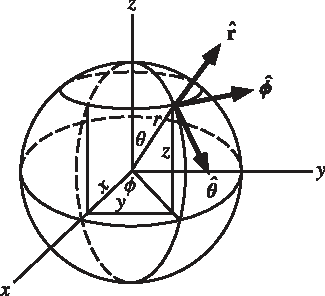
\includegraphics{./figure/math/SphericalCoordinates.pdf}
        \caption{球坐标系}
        \label{fig:SphererCoord} 
    \end{minipage}
    \begin{minipage}{0.42\textwidth}
        \centering
        \setlength{\abovecaptionskip}{0.2cm}
        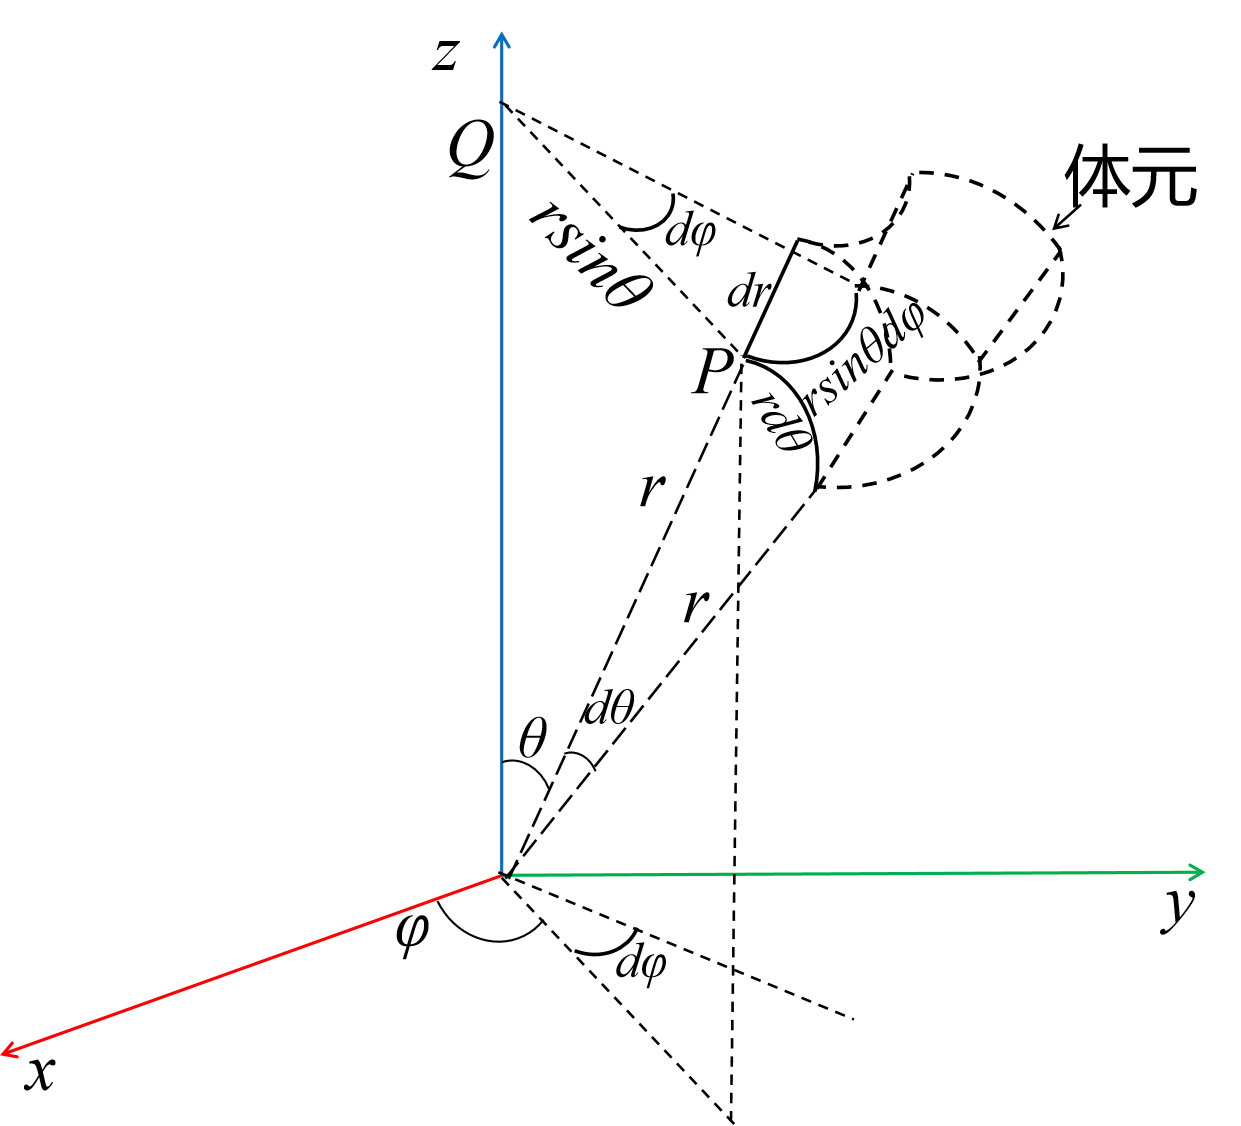
\includegraphics[scale = 0.125]{./figure/math/sphere-vol-ele.png}
        \caption{球坐标系体积元}
        \label{fig:Spherer-Volele} 
    \end{minipage}
\end{figure}

\paragraph*{体积元}
体积元近似为一立方体,然后求其边长
\begin{itemize}
    \item 矢量在$r$方向的偏移为$dr$
    \item 矢量在$\theta$方向的微小偏移:$r\cdot  d\theta$
    \item 矢量在$\phi$方向的微小偏移相当于矢量在$xOy$平面上的投影$r\sin{\theta}$的偏移:$r\sin\theta\cdot d\phi$
\end{itemize}
最后得到体积元公式为
\begin{equation}
    dV = r^2 \sin{\theta} d\,r\ d\,\theta d\,\phi
\end{equation}

\paragraph*{球坐标到Cartesian坐标的转换}
球坐标上某一点$\vbP(r, \theta, \phi)$变换到Cartesian坐标的变换公式为
\begin{equation}
    \begin{aligned}
        \vbe_{x} 
       &= \vbe_{r}\sin\theta\cos\phi + \vbe_{\theta}\cos\theta\cos\phi - \vbe_{\phi}\sin{\phi} \\
        \vbe_{y} 
       &= \vbe_{r}\sin\theta\sin\phi + \vbe_{\theta}\cos\theta\sin\phi + \vbe_{\phi}\cos{\phi} \\
        \vbe_{z} 
       &= \vbe_{r}\cos\theta - \vbe_{\theta}\sin\theta
    \end{aligned}
    \label{eq:sphere-to-cartesian}
\end{equation}
写成矩阵形式为


%%%%%%%%%%%%%%%%%%%%%%%%%%%%%%%%%%%%%%%%%%%%%%%%%%%%%%%%%%%%%%%%%%%%%
\subsection{球坐标下的\texorpdfstring{$\nabla$}{}算符}
球坐标系下的$\nabla$算符可写为:
\begin{equation}
    \nabla =  \vbe_r \frac{\partial}{\partial r} 
            + \vbe_\theta \frac{\partial}{\partial \theta}
            + \vbe_\phi \frac{1}{r\sin{\theta}} \frac{\partial}{\partial \phi}
    \label{eq:nabla-sphere-form}
\end{equation}

球坐标系下标量场$T$和矢量场$\vbv$,矢量导数的坐标表示为,\newline
梯度:
\begin{equation}
    \nabla T = \frac{\partial T}{\partial r} \vec{\bm{e}}_r
              +\frac{1}{r} \frac{\partial T}{\partial \theta} \vbe_{\theta}
              +\frac{1}{r\sin{\theta}}\frac{\partial T}{\partial \phi} \vbe_{\phi}
    \label{eq:sphere-gradient}
\end{equation}
散度:
\begin{equation}
    \nabla \cdot \vbv = \frac{1}{r^2} \frac{\partial}{\partial r}(r^2 v_r)
      + \frac{1}{r\sin{\theta}}\frac{\partial}{\partial\theta}(\sin{\theta}\, v_{\theta})
      + \frac{1}{r\sin{\theta}}\frac{\partial}{\partial\phi} v_{\phi}
    \label{eq:sphere-divergence}
\end{equation}
旋度:
\begin{equation}
    \nabla \times \vec{\bm{v}} =
    \frac{1}{r\sin{\theta}}\left[ \frac{\partial}{\partial\theta}(\sin{\theta}\,v_{\phi}) 
                      - \frac{\partial v_{\theta}}{\partial\phi}\right] \vbe_r
     +\frac{1}{r} \left[ \frac{1}{\sin{\theta}} \frac{\partial v_{r}}{\partial \phi} 
                 - \frac{\partial}{\partial r}(r v_{\phi})\right] \vbe_{\theta}
     +\frac{1}{r}\left[\frac{\partial}{\partial r}(r v_{\theta})
                 - \frac{\partial v_{r}}{{\partial \theta}} \right] \vbe_{\phi}
    \label{eq:sphere-curl}
\end{equation}

%%%%%%%%%%%%%%%%%%%%%%%%%%%%%%%%%%%%%%%%%%%%%%%%%%%%%%%%%%%%%%%%%%%%%
\section{矢量与标量的分类}
%%%%%%%%%%%%%%%%%%%%%%%%%%%%%%%%%%%%%%%%%%%%%%%%%%%%%%%%%%%%%%%%%%%%%
三维Cartesian坐标系中,定义宇称变换矩阵
\begin{equation}
    \bmP = \begin{pmatrix}
        -1  &   0   &   0   \\
         0  &  -1   &   0   \\
         0  &   0   &  -1 
    \end{pmatrix}
    \label{eq:inverse-matrix}
\end{equation}
其表示对坐标取负:$x\rightarrow -x$、$y\rightarrow -y$和$z\rightarrow -z$。通过上述变换矩
阵,我们可以将矢量分为\textbf{极矢量(polar vectors)}、\textbf{赝矢量(pseudovectors)或轴矢
量(axial vectors)};标量分为\textbf{标量(scalar)}、\textbf{赝标量(pseudoscalar)}。

\paragraph*{极矢量}
对任意矢量$\vbV$,若宇称变换矩阵$\bmP$作用后使其符号发生改变,将其定义为极矢量,如下:
\begin{equation}
    \bmP \vbV = -\vbV
    \label{eq:polar-vector}
\end{equation}
如位置矢量$\vbr$和速度矢量$\vbv$。

\paragraph*{赝矢量(轴矢量)}
赝矢量定义为两个极矢量的叉乘
\begin{equation}
    \vbV^{\ast} = \vbV_1 \times \vbV_2
    \label{eq:pesudovectors-def}
\end{equation}
如角动量$\vbl = \vbr \times \vbp$就是赝矢量,其特征就是当宇称矩阵$\bmP$作用其上不改变它的
符号:
\begin{equation}
    \bmP \vbV^{\ast} = (\bmP \vbV_1) \times (\bmP \vbV_1) = \vbV^{\ast}
    \label{eq:pesudovec-parity}
\end{equation}
例如,角动量$\vbl = \vbr \times \vbp$是一个赝矢量,它由位置矢量$\vbr$和动量矢量$\vbp$这两
个矢量的叉乘得到,当宇称变换矩阵作用上去后,位置矢量和动量矢量符号都发生了改变,故最后得到
的角动量符号不发生变化。
\begin{note}
    若宇称算符作用在坐标轴上,虽然赝矢量的符号不变,但它相对坐标轴的方向确实是变化了的;若
    坐标轴发生变化,则整个坐标系统从右手系变到了左手系。
\end{note}

\paragraph*{标量}
标量$S$定义为
\begin{equation}
    \bmP S = S
    \label{eq:scalar-def}
\end{equation}
也就是说标量仅有大小而没有方向。

\paragraph*{赝标量}
赝标量$S^{\ast}$定义为
\begin{equation}
    S^{\ast} = \vbV \cdot \vbV^{\ast}
    \label{eq:pseudoscalar-def}
\end{equation}
如此,宇称变换算符$\bmP$作用后,赝标量符号改变
\begin{equation}
    \bmP S^{\ast} = \bmP (\vbV \cdot \vbV^{\ast}) = (\bmP \vbV) \cdot (\bmP\vbV^{\ast})
                  = -\vbV \cdot \vbV^{\ast} = -S^{\ast}
    \label{eq:pseudoscalar-prop1}
\end{equation}


%%%%%%%%%%%%%%%%%%%%%%%%%%%%%%%%%%%%%%%%%%%%%%%%%%%%%%%%%%%%%%%%%%%%%
\section{矢量场理论}
%%%%%%%%%%%%%%%%%%%%%%%%%%%%%%%%%%%%%%%%%%%%%%%%%%%%%%%%%%%%%%%%%%%%%
\paragraph{势函数}
若一个矢量场$\vbF$的旋度处处为0,则$\vbF$可表示为一个标量势$V$的梯度
\begin{equation}
    \nabla \times \vbF = 0 \Leftrightarrow \vbF = -\nabla V
    \label{eq:scalar-poten}
\end{equation}
\begin{proof}
    必要性,上面左边等式
    \begin{equation*}
        \vbF = - \nabla V = -\vbe_x \frac{\partial V_x}{\partial x}
                            -\vbe_y \frac{\partial V_y}{\partial y}
                            -\vbe_z \frac{\partial V_z}{\partial z}
    \end{equation*}
    因此有
    \begin{equation*}
        \nabla \times \vec{\bm{F}} = \left|\begin{matrix}
            \vbe_x  &   \vbe_y  &   \vbe_z  \\
            \frac{\partial}{\partial x} & \frac{\partial}{\partial y} & \frac{\partial}{\partial z} \\
            -\frac{\partial V}{\partial x} & -\frac{\partial V}{\partial y} & -\frac{\partial V}{\partial z}
        \end{matrix}\right|
        = 0
    \end{equation*}
    充分性,待补充。
\end{proof}

\begin{theorem}[无旋场]
    以下条件等价:
    \begin{enumerate}
        \item 对任何一点满足$\nabla \times \vbF = 0$;
    \end{enumerate}
\end{theorem}

%%%%%%%%%%%%%%%%%%%%%%%%%%%%%%%%%%%%%%%%%%%%%%%%%%%%%%%%%%%%%%%%%%%%%
\section{一些重要结论}
%%%%%%%%%%%%%%%%%%%%%%%%%%%%%%%%%%%%%%%%%%%%%%%%%%%%%%%%%%%%%%%%%%%%%
列出一些经常用到的公式计算结果及证明.